\documentclass{ctexbeamer}
\usepackage{ctex}
\usepackage{tikz}
\usepackage{minted}

\title{TikZ绘图基础讲解}
\begin{document}

\begin{frame}[fragile]{绘制点}
    \begin{itemize}
        \item 使用 \texttt{(x,y)} 坐标来绘制点
    \end{itemize}
    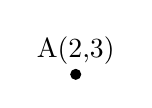
\begin{tikzpicture}
        % 绘制一个点
        \fill (2,3) circle (2pt);  % 绘制坐标 (2,3) 的点
        % 标注点坐标
        \node at (2,3.3) {A(2,3)};
    \end{tikzpicture}
    \begin{minted}[frame=single,framesep=10pt]{latex}
    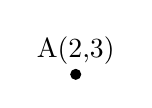
\begin{tikzpicture}
        % 绘制一个点
        \fill (2,3) circle (2pt);  % 绘制坐标 (2,3) 的点
        % 标注点坐标
        \node at (2,3.3) {A(2,3)};
    \end{tikzpicture}
    \end{minted}
\end{frame}

\begin{frame}[fragile]{绘制三角形}
    \begin{itemize}
        \item 三角形可以通过三个点连接
    \end{itemize}
    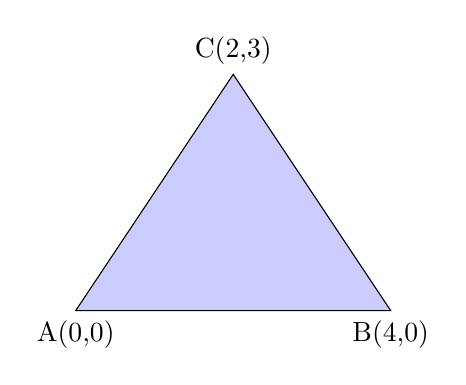
\begin{tikzpicture}
        % 绘制三角形
        \draw[fill=blue!20] (0,0) -- (4,0) -- (2,3) -- cycle;
        % 标注顶点
        \node at (0,-0.3) {A(0,0)};
        \node at (4,-0.3) {B(4,0)};
        \node at (2,3.3) {C(2,3)};
    \end{tikzpicture}
    \begin{minted}[frame=single,framesep=10pt]{latex}
    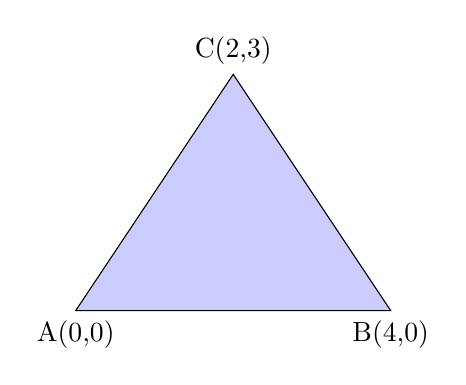
\begin{tikzpicture}
        % 绘制三角形
        \draw[fill=blue!20] (0,0) -- (4,0) -- (2,3) -- cycle;
        % 标注顶点
        \node at (0,-0.3) {A(0,0)};
        \node at (4,-0.3) {B(4,0)};
        \node at (2,3.3) {C(2,3)};
    \end{tikzpicture}
    \end{minted}
\end{frame}

\begin{frame}[fragile]{绘制长方形}
    \begin{itemize}
        \item 长方形通过两个对角点确定
    \end{itemize}
    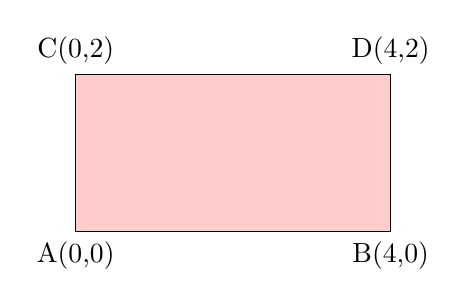
\begin{tikzpicture}
        % 绘制长方形
        \draw[fill=red!20] (0,0) rectangle (4,2);
        % 标注顶点
        \node at (0,-0.3) {A(0,0)};
        \node at (4,-0.3) {B(4,0)};
        \node at (0,2.3) {C(0,2)};
        \node at (4,2.3) {D(4,2)};
    \end{tikzpicture}
    \begin{minted}[frame=single,framesep=10pt]{latex}
    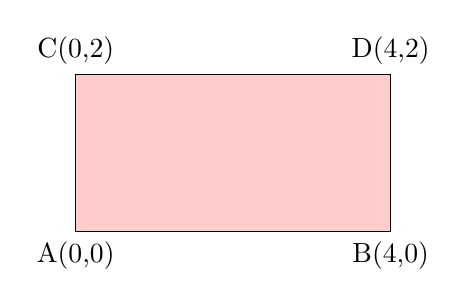
\begin{tikzpicture}
        % 绘制长方形
        \draw[fill=red!20] (0,0) rectangle (4,2);
        % 标注顶点
        \node at (0,-0.3) {A(0,0)};
        \node at (4,-0.3) {B(4,0)};
        \node at (0,2.3) {C(0,2)};
        \node at (4,2.3) {D(4,2)};
    \end{tikzpicture}
    \end{minted}
\end{frame}

\begin{frame}[fragile]{绘制圆和椭圆}
    \begin{itemize}
        \item 使用 \texttt{circle} 绘制圆形,使用 \texttt{ellipse} 绘制椭圆
    \end{itemize}
    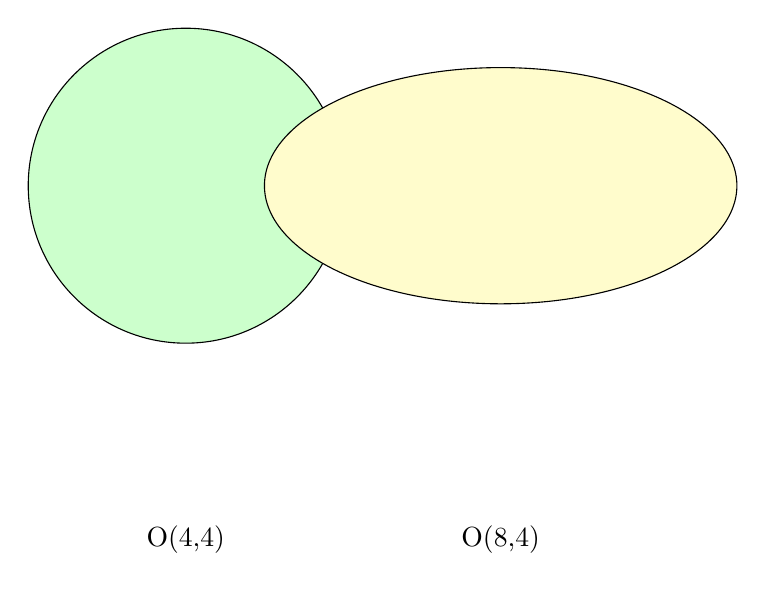
\begin{tikzpicture}
        % 绘制圆形
        \draw[fill=green!20] (4,4) circle(2cm);
        \node at (4,-0.5) {O(4,4)};
        % 绘制椭圆
        \draw[fill=yellow!20] (8,4) ellipse (3cm and 1.5cm);
        \node at (8,-0.5) {O(8,4)};
    \end{tikzpicture}
    \begin{minted}[frame=single,framesep=10pt]{latex}
    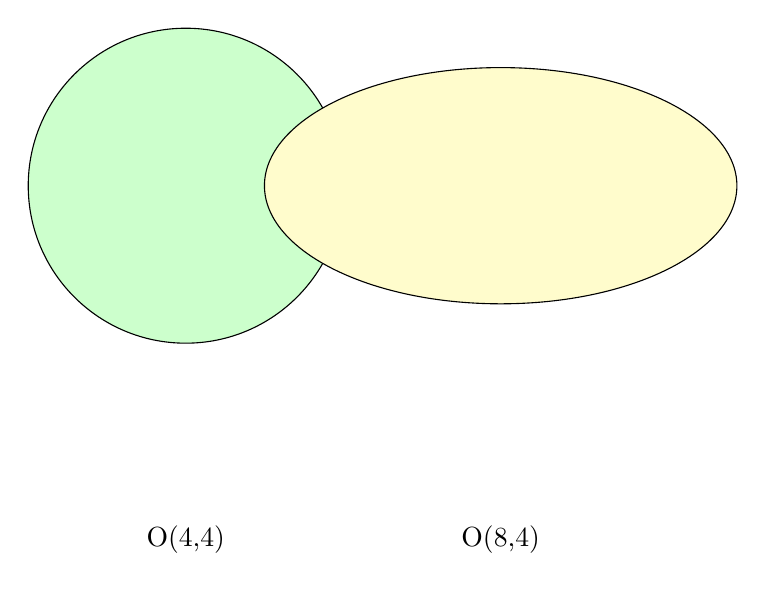
\begin{tikzpicture}
        % 绘制圆形
        \draw[fill=green!20] (4,4) circle(2cm);
        \node at (4,-0.5) {O(4,4)};
        % 绘制椭圆
        \draw[fill=yellow!20] (8,4) ellipse (3cm and 1.5cm);
        \node at (8,-0.5) {O(8,4)};
    \end{tikzpicture}
    \end{minted}
\end{frame}

\begin{frame}[fragile]{绘制圆弧}
    \begin{itemize}
        \item 圆弧使用 \texttt{arc} 命令绘制
    \end{itemize}
    \begin{tikzpicture}
        % 绘制圆弧
        \draw (0,0) arc[start angle=0, end angle=90, radius=2cm];
        \node at (2.5,-0.5) {圆弧(0°, 90°)};
    \end{tikzpicture}
    \begin{minted}[frame=single,framesep=10pt]{latex}
    \begin{tikzpicture}
        % 绘制圆弧
        \draw (0,0) arc[start angle=0, end angle=90, radius=2cm];
        \node at (2.5,-0.5) {圆弧(0°, 90°)};
    \end{tikzpicture}
    \end{minted}
\end{frame}

\end{document}
